%%%%%%%%%%%%%%%%%%%%%%%%%%%%%%%%%%%%%%%%%%%%%%%%%%%%%%%%%%%%%%%%%%%%%%%%%%%%%%%%
%2345678901234567890123456789012345678901234567890123456789012345678901234567890
%        1         2         3         4         5         6         7         8

\documentclass[letterpaper, 10 pt, conference]{ieeeconf}  % Comment this line out if you need a4paper

%\documentclass[a4paper, 10pt, conference]{ieeeconf}      % Use this line for a4 paper

\IEEEoverridecommandlockouts                              % This command is only needed if 
                                                          % you want to use the \thanks command

\overrideIEEEmargins                                      % Needed to meet printer requirements.

%In case you encounter the following error:
%Error 1010 The PDF file may be corrupt (unable to open PDF file) OR
%Error 1000 An error occurred while parsing a contents stream. Unable to analyze the PDF file.
%This is a known problem with pdfLaTeX conversion filter. The file cannot be opened with acrobat reader
%Please use one of the alternatives below to circumvent this error by uncommenting one or the other
%\pdfobjcompresslevel=0
%\pdfminorversion=4

% See the \addtolength command later in the file to balance the column lengths
% on the last page of the document

% The following packages can be found on http:\\www.ctan.org
%\usepackage{graphics} % for pdf, bitmapped graphics files
%\usepackage{epsfig} % for postscript graphics files
%\usepackage{mathptmx} % assumes new font selection scheme installed
%\usepackage{times} % assumes new font selection scheme installed
%\usepackage{amsmath} % assumes amsmath package installed
\usepackage{amssymb}  % assumes amsmath package installed
\usepackage{amscd,amsmath}
\usepackage{amsfonts}
\usepackage{biblatex}
\usepackage{csvsimple}
\usepackage{pgfplots}
\usepackage{pgfplotstable}
\usepackage{hyperref}
\usepackage{algorithm}
\usepackage{algpseudocode}
\usepackage{rotating}
\usepackage{gensymb}
%\pgfplotsset{compat=1.7}
\usepackage{graphicx}
\usepackage{import}
\usepackage{placeins}
\usepgfplotslibrary{external} 
\tikzexternalize

\newcommand\norm[1]{\left\lVert#1\right\rVert}

\title{\LARGE \bf
Fault Detection of Sun Reflection to Increase Estimation Accuracy of Satellite Attitude
}


\author{Louw UJ$^{1}$, Jordaan HW$^{2}$, Schoeman JC$^{3}$% <-this % stops a space
\thanks{*This work was not supported by any organization}% <-this % stops a space
\thanks{$^{1}$Louw UJ is with Faculty of Electronic \& Electrical Engineering, Electronic System            Laboratory, University of Stellenbosch, Stellenbosch Central, Stellenbosch, 7600
        {\tt\small louwuj@gmail.com}}%
}

\addbibresource{bibliography.bib} 

\begin{document}



\maketitle
\thispagestyle{empty}
\pagestyle{empty}


%%%%%%%%%%%%%%%%%%%%%%%%%%%%%%%%%%%%%%%%%%%%%%%%%%%%%%%%%%%%%%%%%%%%%%%%%%%%%%%%
\begin{abstract}

The Kalman Filter is a state estimator that is often used in attitude determination of satellites. A Kalman filter is highly sensitive to anomalies that occur in sensors. A good example of this is the reflection of a solar panel on a sun sensor that changes the perceived sun vector. This in term influences the estimation of the attitude by the kalman filter and consequently the control of the satellite. Detecting anomalies in sensors and omitting the sensor reading from the measurement update of the Kalman Filter could increase the stability and reliability of the Kalman filter for satellite attitude determination.

\emph{keywords} --- anomaly detection, Kalman filter, machine learning, sun reflection, satellites, sensors

\end{abstract}


%%%%%%%%%%%%%%%%%%%%%%%%%%%%%%%%%%%%%%%%%%%%%%%%%%%%%%%%%%%%%%%%%%%%%%%%%%%%%%%%
\section{INTRODUCTION}

For many satellite missions the attitude determination is of high importance. A mission that requires earth following during eclipse and otherwise sun following for solar charging requires accurate attitude estimation. The focus of this article is the attitude determination and control system \emph{ADCS} of the satellite. This system is demonstrated in Figure~\ref{fig:System_Diagram}. The current state vector of the system can not be determined with only the use of models or sensors. Since the sensors contains noise and the mathematical model does not include certain disturbances in the actual system. Therefore a probabilistic approach can be used to determine the state vector with the highest probability. 

An Extended Kalman Filter (\emph{EKF}) is a common estimator used in satellite missions. The EKF is a method which incorporates a physics based model of the satellite dynamics as well as using sensor fusion and measurement updates to ensure accurate estimation. The sensor measurements that are used for the measurement update, are the sensors that provide a modelled ORC vector as well as measured SBC vector, such as the magnetometer, sun sensor, nadir sensor and star tracker. The noise of the measurements and the noise of the system is incorporated in the EKF model to ensure stability and reliable estimation. The general principal for measurement updates, is to update the EKF from the least to the most reliability measurements. The error between the modelled and measured vectors are used to update the EKF estimation. The EKF and the specific configuration thereof for satellites can be researched further from \textcite{JansevanVuuren2015}. 

The problem with an EKF is when the sensors do not follow their modelled vector. Slight deviations thereof won't have significant effects, but anomalies such as failed sensors can cause the EKF to become unstable. Consequently, we want to be able to recover from failed sensors. The frequency of the anomaly occurrence can also determine the stability of the Kalman filter. Therefore we opted to use sun reflection from solar panel on sun sensors as our modelled anomaly. This is a real problem in the satellite industry which can be isolated with changes in the satellite design. However, with an inadequate design the problem can manifold when the satellite design is used on a satellite constellation. 

This anomaly also requires autonomous decision making, since the control of the satellite to be sun facing cannot be done by the ground station during orbit and is highly determined by the sun vector. Therefore we aim to design a fault detection, isolation and recovery system specifically for the sensor anomalies and the testing thereof will be done on the solar reflection anomaly. The specific use case will be a mission that requires earth following during eclipse and sun following otherwise on a generic small satellite design as seen in Figure~\ref{fig:CubeSat}.

\begin{figure*}[h!b!t]
	\centering
	\def\svgwidth{12cm}
	\import{Figures/}{Control_Diagram.pdf_tex}
	\caption{System Diagram}
	\label{fig:System_Diagram}
\end{figure*}

\subsection{Related Work}
Sun failures are not a new problem and has consequently been researched thoroughly. Hardware solutions to sun reflection have been developed with the use of digital sun sensors that can discriminate between direct sunlight and reflected sunlight. These digital sun sensors however, are not as accurate as many other analog sun sensors. There is also a long list of research that has been done with regards to sensor fault detection (as seen in \cite{wang2019adaptive}). One of the most relevant articles is done by \textcite{wang2019adaptive}, and proposed a adaptive unscented Kalman filter for sensor fault estimation and isolation. The results thereof seems promising and is based on dramatical changes in the measurements. However, even for sun reflection, the measurement change occurs often and the control of the satellite also changes with it. Therefore future work might be to use the algorithm developed by \textcite{wang2019adaptive} to test the response thereof on sun reflection.

Other research that is used for feature extraction in this article is based on research done by \textcite{DeSilva2020}. Fault prediction is done by implementing an innovative moving average, determined by the error estimated by a dynamic mode decomposition and a kalman filter, as a input to a predictive model --- decision tree. The method is tested on various physics based models.

\subsection{Preliminaries}
The details of satellite dynamics will not be discussed in this article, however it must be noted that orbit-reference coordinate and satellite body coordinate frame will be referred to as \emph{ORC} and \emph{SBC} respectively. General notation of this article will be matrices, as a upper-case letter in bold, $\mathbf{A}$, vectors, as lower case letters in bold, $\mathbf{a}$ and scalar values as lower case letters, $a$. All vectors values will be given in the order $[x, y, z]$.

\section{Reflection}
\label{section:Reflection}
The reflection anomaly is modelled for any dimensions but with the specific shape and design of the cubesat as shown in Figure~\ref{fig:CubeSat}.

\begin{figure}[!htb]
	\centering
	\def\svgwidth{7cm}
	\import{Figures/}{ReflectionModel.pdf_tex}
	\caption{Cube Sat}
	\label{fig:CubeSat}
\end{figure}

\begin{figure*}[!hbt]
	\centering
	\def\svgwidth{7cm}
	\import{Figures/}{ReflectionModelPoint.pdf_tex}
	\centering
	\def\svgwidth{7cm}
	\import{Figures/}{LineIntersection.pdf_tex}
	\caption{Reflection}
	\label{fig:LineIntersection}
\end{figure*}

The assumption is made that the solar panel can be modelled as a plane. Therefore light that hits the solar panel will reflect as if it hits a perfectly smooth mirror. It is also assumed that if any reflection from the solar panel hits the sun sensor, the sun sensor will then default to the reflection ray instead of the modelled sun vector. The reflected sun vector, $R$, can be calculated as
\begin{equation}
	R = V - 2N^T(V \cdot N)
\end{equation}
Where $V$ is the incoming sun vector and $N$ is the normal vector to the plane $ABCD$ of the solar panel as seen in Figure~\ref{fig:CubeSat}. To calculate the intersection of the reflected vector with the plane $XWYZ$ of the sun sensor the intersecting point the equation of the plane, reflected vector and the point of origin is required. The equation for a plane can be denoted as 

\begin{equation}
	P = ax + by + cz = d
	\label{eq:Plane}
\end{equation}
where $x, y and z$ are the dimensions in the SBC frame. The reflected unit vector can also be translated to 

\begin{equation}
	\begin{aligned}
	&	x = \alpha t \\
	&	y = \beta t \\
	&	z = \zeta t \\
	\end{aligned}
\label{eq:LineOfVector}
\end{equation}
where the coefficients, $\alpha$, $\beta$ and $\zeta$ are the values of the reflected unit vector in each respective dimension. Since we can calculate the coefficients for Eq~\ref{eq:LineOfVector} from the reflected vector, we can calculate $t$, by substituting $x, y \& z$ into Eq~\ref{eq:Plane}. This can be done since we determine the equation of the plane for the surface $XYZW$ based on our design. Thereafter, the intersecting point with the plane $XYZW$ can be calculated as

\begin{equation}
	P(x, y, z) = (o_1 + \alpha t, o_2 + \beta t, o_3 + \zeta t)
	\label{eq:Intersection}
\end{equation}
where $o_1, o_2, o_3$ is the position of origin. Which in this case is the position of reflection from the solar panel. Therefore, if the sun vector $\mathbf{v}$ reflected from the solar panel as $\mathbf{r}$, the point of intersection $Q'$ can be calculated as

\begin{equation}
	Q'(x, y, z) = (Q_x + \alpha t, Q_y + \beta t, Q_z + \zeta t)
	\label{eq:SpecificIntersection}
\end{equation}

To model reflection from the solar panels to the sun sensor only two corners of the solar panel and two corners of the sun sensor are to be taken into account. From Figure~\ref{fig:ReflectionPoints} it is evident that if the solar panel reflects on $Y$ that the reflection will also cover $X$. The same is true for corner $Z$ and $W$. Since $C'$ will be at the exact same position as $C$, which is also true for $D'$ and $D$, the calculation thereof can be omitted. Therefore it is only necessary to calculate the reflected positions $A'$ and $B'$. This simplifies the reflection model significantly.

The reflected position $A'$ can be calculated as the intersection of the reflected vector $R$ with plane $XYZW$ using Eq~\ref{eq:Intersection}. We also know the position of $A$, based on the satellite design and can therefore calculate $A'$. The same applies to $B$ and $B'$. To then determine whether $Y$ or $X$ is within the region of reflection, we assume that the plane $XYWZ$ is a 2D plane and we omit the third dimension. Therefore, the axis changes from $x, y, z$ to only $x, y$. We calculate whether $x$ is between the lines of $A'D'$ and $B'C$ as well as between the lines $ACD$ and $A'B'$. By determining the line equation between reflected points in the form 

\begin{equation}
y_{A'B'} = mx_{A'B'} + c
\end{equation}
the corresponding $x$ or $y$ coordinate can be calculated by substituting either $X_y$ or $X_x$ in the line equation. With this the coordinates of $X_{B'C}$, $X_{A'D}$, $X_{A'B}$ and $X_{CD}$ can be determined. Thereafter with logical if statements it can be determined whether $X$ is in the reflection zone. This is demonstrated with the logical that if $X_x$ is to the right of $X_{B'C,x}$ and to the left of $X_{A'D,x}$, as well as $X_y$ is to the above of $X_{A'B',y}$ and below of $X_{CD,y}$ then $X$ is within the reflection zone. 

The results for the sun vector with and without reflection is shown in Figure~\ref{fig:Sun Vector comparison}. For modelling purposes, the reflection in this example has no influence on the estimation and control of the satellite.

\begin{figure*}[!htb]
	\hspace{1cm}
	\begin{tikzpicture}
	%\centering
	\begin{axis}[width = 7cm, ylabel = $\theta$ (deg), y label style = {at={(0,0.5)},
			anchor=north}, xlabel = Time (s), forget plot style={opacity=0.2}, title = Sun vector with reflection]
		
		\addplot[line width=1pt,color=blue, each nth point=10, draw opacity=0.5,filter discard warning=false, unbounded coords=discard] table [x expr=\coordindex, y=Sun_x, col sep=comma]{/home/ulrich/Documents/Masters thesis/Satellite/Data files/pgfPlots/Predictor-PERFECT/Isolator-PERFECT/Recovery-EKF/EARTH_SUN/General CubeSat Model/2Sensors/Reflection.csv};
		\addplot[line width=1pt,color=red, each nth point=10, draw opacity=0.5,filter discard warning=false, unbounded coords=discard] table [x expr=\coordindex, y=Sun_y, col sep=comma]{/home/ulrich/Documents/Masters thesis/Satellite/Data files/pgfPlots/Predictor-PERFECT/Isolator-PERFECT/Recovery-EKF/EARTH_SUN/General CubeSat Model/2Sensors/Reflection.csv};
		\addplot[line width=1pt,color=green, each nth point=10, draw opacity=0.5,filter discard warning=false, unbounded coords=discard] table [x expr=\coordindex, y=Sun_z, col sep=comma]{/home/ulrich/Documents/Masters thesis/Satellite/Data files/pgfPlots/Predictor-PERFECT/Isolator-PERFECT/Recovery-EKF/EARTH_SUN/General CubeSat Model/2Sensors/Reflection.csv};
	\end{axis}
	%\end{tikzpicture}
%	\caption[Sun vector]{Sun vector  with reflection.}
%	\label{fig:Sun Vector with Reflection}
	%\centering
	%\begin{tikzpicture}
		%\centering
		\hspace{7cm}
		\begin{axis}[width = 7cm, xlabel = Time (s), legend style={draw = none, at={(1.15,0.65)},
				anchor=north}, forget plot style={opacity=0.2}, title = Sun vector without reflection]
			
			\addplot[line width=1pt,color=blue, each nth point=10, draw opacity=0.5,filter discard warning=false, unbounded coords=discard] table [x expr=\coordindex, y=Sun_x, col sep=comma]{/home/ulrich/Documents/Masters thesis/Satellite/Data files/pgfPlots/Predictor-None/Isolator-None/Recovery-None/EARTH_SUN/General CubeSat Model/2Sensors/None.csv};
			\addplot[line width=1pt,color=red, each nth point=10, draw opacity=0.5,filter discard warning=false, unbounded coords=discard] table [x expr=\coordindex, y=Sun_y, col sep=comma]{/home/ulrich/Documents/Masters thesis/Satellite/Data files/pgfPlots/Predictor-None/Isolator-None/Recovery-None/EARTH_SUN/General CubeSat Model/2Sensors/None.csv};
			\addplot[line width=1pt,color=green, each nth point=10, draw opacity=0.5,filter discard warning=false, unbounded coords=discard] table [x expr=\coordindex, y=Sun_z, col sep=comma]{/home/ulrich/Documents/Masters thesis/Satellite/Data files/pgfPlots/Predictor-None/Isolator-None/Recovery-None/EARTH_SUN/General CubeSat Model/2Sensors/None.csv};
			\legend{x, y, z}
		\end{axis}
	\end{tikzpicture}
\caption[Sun vector]{Sun vector without reflection.}
\label{fig:Sun Vector comparison}
\end{figure*}

%\begin{figure}[!htb]
%	\centering
%	\begin{tikzpicture}
%		\centering
%		\begin{axis}[width = 7cm, ylabel = $\theta$ (deg), xlabel = Time (s), legend style={draw = none, at={(1.15,0.65)},
%				anchor=north}, forget plot style={opacity=0.2}, title = Sun vector without reflection]
%			
%			\addplot[line width=1pt,color=blue, each nth point=10, draw opacity=0.5,filter discard warning=false, unbounded coords=discard] table [x expr=\coordindex, y=Sun_x, col sep=comma]{/home/ulrich/Documents/Masters thesis/Satellite/Data files/pgfPlots/Predictor-None/Isolator-None/Recovery-None/EARTH_SUN/General CubeSat Model/2Sensors/None.csv};
%			\addplot[line width=1pt,color=red, each nth point=10, draw opacity=0.5,filter discard warning=false, unbounded coords=discard] table [x expr=\coordindex, y=Sun_y, col sep=comma]{/home/ulrich/Documents/Masters thesis/Satellite/Data files/pgfPlots/Predictor-None/Isolator-None/Recovery-None/EARTH_SUN/General CubeSat Model/2Sensors/None.csv};
%			\addplot[line width=1pt,color=green, each nth point=10, draw opacity=0.5,filter discard warning=false, unbounded coords=discard] table [x expr=\coordindex, y=Sun_z, col sep=comma]{/home/ulrich/Documents/Masters thesis/Satellite/Data files/pgfPlots/Predictor-None/Isolator-None/Recovery-None/EARTH_SUN/General CubeSat Model/2Sensors/None.csv};
%			\legend{x, y, z}
%		\end{axis}
%	\end{tikzpicture}
%	\caption[Sun vector]{Sun vector.}
%	\label{fig:Sun Vector comparison}
%\end{figure}

\section{Anomaly Detection}
To be able to recover from sensor anomalies or to exclude the sensor from the kalman filter, the anomaly must be detected and the sensor from which the anomaly in the data occurs must be classified.

\subsection{Feature Extraction}
The first step to implementing a FDIR for kalman filter robustness is to detect whether an anomaly has occured on one of the filters. There are various different methods for fault detection, with both supervised and unsupervised methods. However this study will only focus on a single method proposed by \textcite{DeSilva2020} to detect failures in sensors.

The proposed method by \textcite{DeSilva2020} uses Dynamic Mode Decomposition (DMD), which was originally developed by \textcite{schmid2011applications} and further expanded to include control by \textcite{proctor2016dynamic}, to provide an estimation of a sensor vector based on the previous measurement fo the sensor as well as the measurements of the other sensors in the system. DMD was first developed in the fluids community and constructs a matrix $\mathbf{A}$ to relate the state vector $x$ with the following time step of the state vector, $x_{k+1}$. The state vector in our case will be the measurement vector of the specific sensor that we want to monitor.
\begin{equation}
	x_{k+1} = \mathbf{A}x_k
\end{equation}
Where $x_k$ and $x_{k+1}$ over a time period will be denoted as $\mathbf{X}$ and $\mathbf{X'}$ respectively.

The method of DMD however is useful for high order systems where the calculation of $\mathbf{A}$ is computation intensive. This is not the case for our system and using DMD is not justifiable. Therefore we calculate the pseudo-inverse of $\mathbf{X}$, denote it as $\mathbf{X^{\dagger}}$, and $\mathbf{A}$ can be calculate as
\begin{equation}
	\mathbf{A} = \mathbf{X}\mathbf{X^{\dagger}}
\end{equation}
This necessitates the required data for the state vector. The article by \textcite{DeSilva2020} however includes the $\mathbf{B}$ to relate the vector measurements of the other sensors to adjust the predicted state, $x_{k+1}$ of the monitored sensor. 
\begin{equation}
	x_{k+1} = \boldsymbol{A}x_k + \boldsymbol{B}y_k
	\label{control DMD}
\end{equation}
Where $y_k$ is the other sensor measurements. This is adjusted for our use case, where $y_k$ is the control inputs for the magnetotorquers and reaction wheels and $x_k$ is all of the sensor measurements. Consequently, the model of \ref{control DMD} denotes the prediction of the sensor measurements in time step $k+1$ based on the current sensor measurements and control inputs.
Thereafter, as implemented by \textcite{DeSilva2020} the model is adjusted by with a Kalman Filter. From $\boldsymbol{A}$ and $\boldsymbol{B}$ the Kalman filter can be implemented to predict $x_{k+1}$
\begin{equation}
	\hat{x}_{k+1} = A\hat{x}_k + By_k + K(x_k - \hat{x}_k)
\end{equation}
After  the calculation of $\hat{x}_{k+1}$ \textcite{DeSilva2020} proposes a moving average of the innovation covariance
\begin{equation}
	\boldsymbol{V}_k = \frac{1}{N} \sum_{i=k-N}^k (x_i - \hat{x}_i)(x_i - \hat{x}_i)^T
\end{equation}
The moving average is used as an additional input parameter for the classification of anomalies based on the $\boldsymbol{x_k}$.

\subsection{Classification}
The first step of FDIR is to classify whether an anomaly exists in the current sensor data. For the proposed method, decision trees will be implemented to classify anomalies. A decision tree is a classification method that splits data samples based on a threshold of a specific input parameter. For instance to split a data samples from both a satellite orbit based on being in an eclipse or not, would be simply to measure whether the sun vector is $0$. With the assumption that the sun sensor has no anomalous behaviour.

However to split the data for the anomalies we need to decide which input parameter will be used to make the first split, root node. The Gini index provides a measure of the probability of a data sample being being wrongly classified at a given node. This can be calculated with Eq~\ref{eq:Gini index}.

\begin{equation}
GI = 1 - \sum_{i = 1}^{n}{(P_i)^2}
\label{eq:Gini index}
\end{equation}

The operator split that produces the lowest Gini index, provides the most pure split and will therefore be used as the root node. For our use case the CART algorithm will be used to optimize the decision tree, which also takes into account the largest information gain to construct the decision tree. Figure~\ref{fig:DecisionTree} is a graphical representation of the decision tree developed to classify anomalies. The depth of a decision tree determines how many splits occur from the root node to the leaf node the furthest from the first split. If the depth is unspecified, the decision tree will split until all the data samples are perfectly split into anomalous and normal data samples. However, the larger the depth, the more bias the decision tree is to the training data. Therefore, the depth is specified to $10$ for our use case.

\begin{figure*}[!htb]
	\centering
	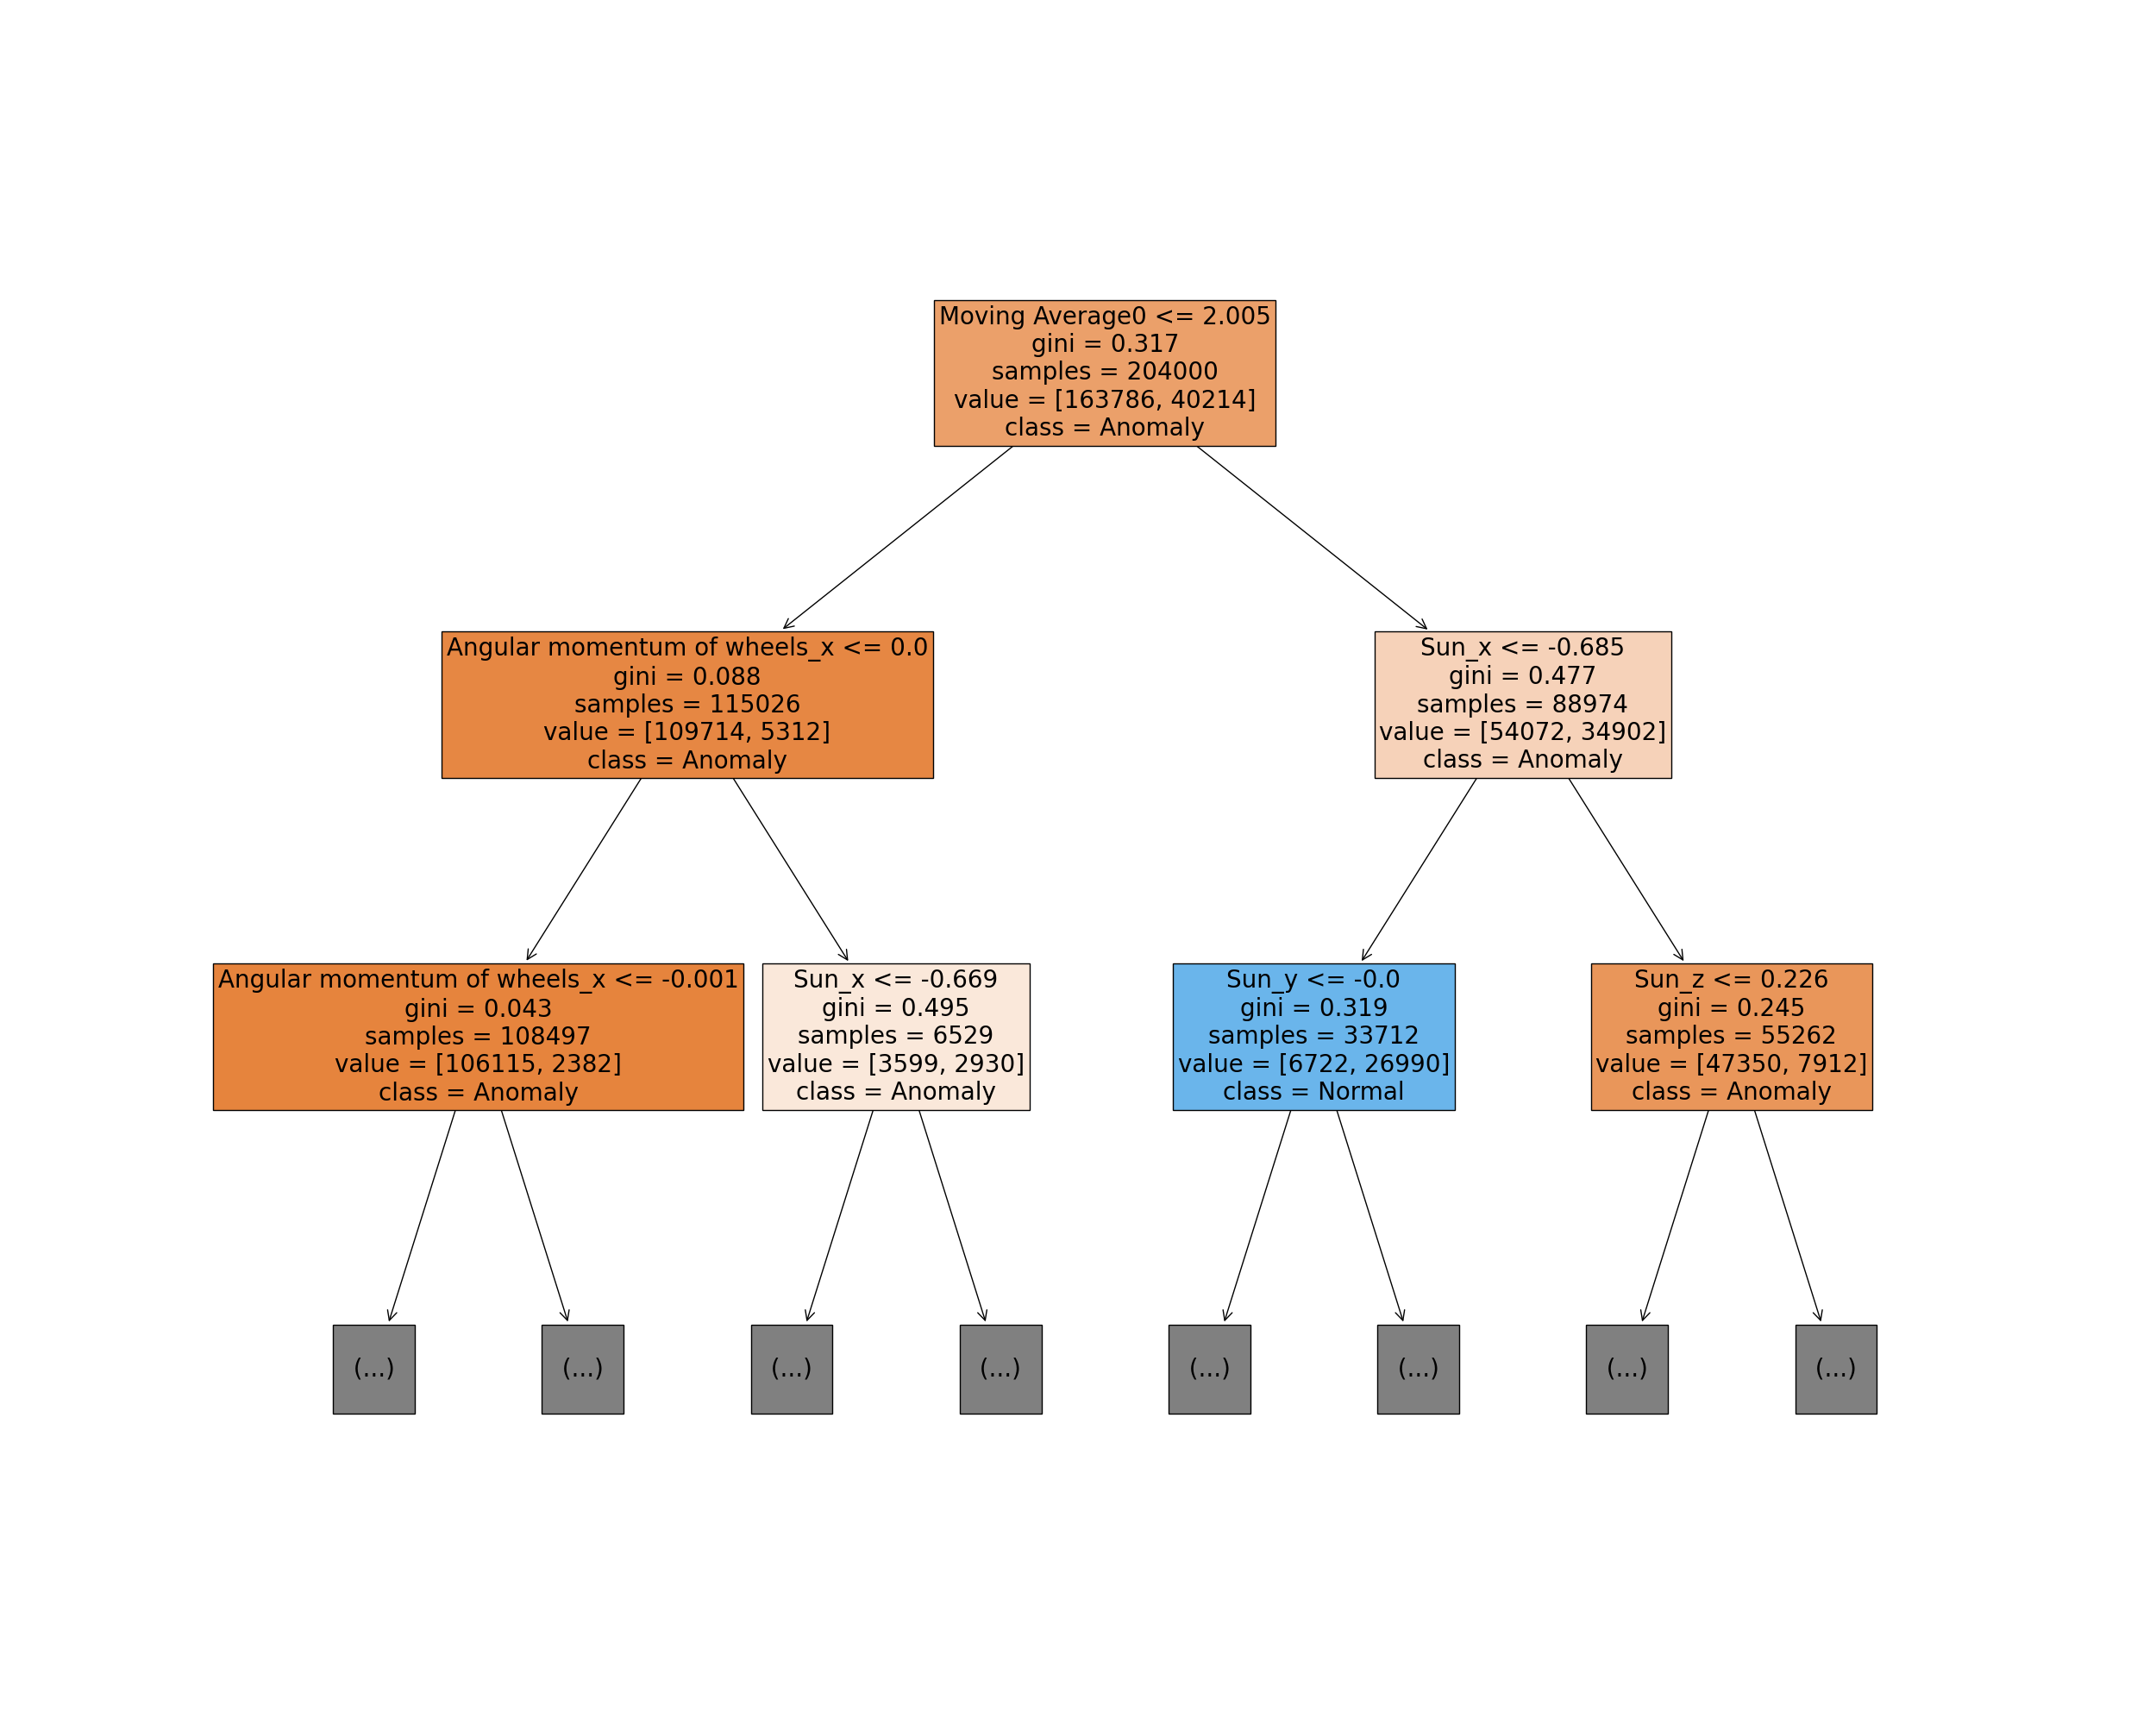
\includegraphics[trim = {3cm 7cm 3cm 7cm},clip, width = 15cm]{/home/ulrich/Documents/Masters thesis/Satellite/Hyperparameters/PhysicsEnabledDMDMethod/DecisionTreeBinaryClass.png}
	\label{fig:DecisionTree}
\end{figure*}

Random Forests, an method of using the prediction average of randomly sampled decision trees, is also tested and the results thereof shown in section~\ref{section:Results}.  


\subsection{Recovery}
Three different methods of recovery are compared. These methods are all focused on ensuring that the sun reflection does not change the reliability and stability of the EKF.

The ignore method uses the detected sensor that has failed and ignores the sensor measurement from the EKF measurement update. This method is based on the assumption that the EKF estimation is correct up until the moment where the sensor failure is detected. This method can also have variations, such as the change of the measurement noise covariance matrix $R_k$. This however will dramatically change $K_k$ and will destabilize the EKF rather than stabilizing it. Both methods results however will be discussed in section~\ref{section:Results}.

The replacement methodology changes $v_{meas,k}$ to $v_{est,k}$ at the timestep when the failure is detected. This method depends on the stability and accuracy of the EKF when the failure is detected and highly depends on the accuracy of the detection method. Although this seems to bypass the entire purpose of a measurement update, and might change the change the EKF's dependency to be more on the sensor than the model, even though the sensor measurement might not be accurate. The EKF will remain stable due to the other measurements being accurate and will save computation time. The EKF will not require any reset and the same number of measurements updates will still occur during a sensor's anomalous behaviour.

The backtrack method uses a buffer of $v_{meas,k}$, $v_{model,k}$ and $\hat{x}_k^+$ and other parameters that are used to update the EKF. If a sensor failure is detected, the sensor is excluded from the EKF and the EKF is updated with the sensor data in the buffer excluding the sensor that has failed. The EKF is therefore \emph{reset} and updated from timestep $t_{k-N}$ to $t_k$, where $N$ is the size of the number of timesteps in the buffer. $N$ however must be optimized based on the computational time used to reset the EKF, but still ensure convergence of the EKF. If the sensor that was detected to have anomalous behaviour changes back to normal again, the EKF will be reset once again and the sensor will only be included in the measurement update of $t_k$ since it was anomalous for timesteps before $t_k$.

A backtrack method can be combined with both the replacement and ignore method. Where the backtrack method is implemented only after a specified number of sun reflections are predicted.

\section{Testing Setup}
To ensure repeatability of the tests conducted in this article, the github repo is provided ...
sgp4 simulation environment. Disturbances. The testing for the FDIR methods is done by implementing a reflection model on a cubesat from the moment of launching the satellite. Therefore the recovery methods are also implemented from the beginning of the satellite orbit. The mission of the ADCS of this specific satellite is to be nadir pointing during eclipse and sun following otherwise.

The simulation is run for 20 orbits, with each orbit running for 5700$s$. If a fault is induced, it is induced after the first two orbits and the specific anomaly then occurs for the following 18 orbits.

\subsection{Control}
Quaternion-feedback control with momentum dumping only during eclipse. The attitude command vector during nadir-pointing in the SBC frame is $\mathbf{u}_c = [0, 0, 1]$, since the SBC frame $z$ coordinate should line up with the ORC frame. During the sun following phase, the attitude command according to \textcite{chen2000ground} can be calculated as 

\begin{equation}
\mathbf{u}_c = \frac{\mathbf{u}_{sp}^{SBC} \times \mathbf{s}_o}{\norm{\mathbf{u}_{sp}^{SBC} \times \mathbf{s}_o}}
\end{equation}

where $\mathbf{s}_o$ is the measured unit sun vector in ORC, and the main solar panel's position is denoted as a unit vector, $\mathbf{u}_{sp}^{SBC}$. The angle between $\mathbf{u}_{sp}^{SBC}$ and $\mathbf{s}_o$, $\delta$, can be calculated with the vector dot-product. The command quaternion $\mathbf{q}_c$ can then be calculated

\begin{equation}
\mathbf{q}_c = \begin{bmatrix}
	\mathbf{u}_c sin(\frac{\delta}{2}) \\
	cos(\frac{\delta}{2})
\end{bmatrix}
\end{equation}
This can then be used as the reference for the control. The reference $\omega_b^I$ is always $[0, 0, 0]$.

\subsection{Dimensions of Satellite}
The dimensions of the satellite are shown in Table~\ref{Table:Dimensions}.

\begin{table}[!htb]
	\caption{\label{Table:Dimensions}Dimensions of Cubesat}
	\begin{tabular}{|c|c|c|c|}
		\hline
		\textbf{Dimensions} & \textbf{Satellite (m)} & \textbf{Solar Panels (m)} & \textbf{Sun Sensor (m)} \\ \hline
		\textbf{x}          & $0.3$                    & $0.3$                       & $0.028$                   \\ \hline
		\textbf{y}          & $0.3$                    & $0.3$                       & $0.023$                   \\ \hline
		\textbf{z}          & $0.4$                    & $0.002$                     & N/A                     \\ \hline
	\end{tabular}
\end{table}
The Sputnix dimensions for the sun sensor are used.
% https://sputnix.ru/en/equipment/cubesat-devices/sun-sensor-flight-proof-1
% https://www.cubesatshop.com/product/nss-cubesat-sun-sensor/

\subsection{Orbit Parameters}
Low earth orbiting ($500$km)

\subsection{Sensors}
The sensors used for the measurement update of the Kalman filter is a magnetometer, nadir sensor, sun sensor and star tracker and the measurement update is also done in the order as listed. This is due to the noise models of the sensors, as all the sensor noise models are based on zero-mean Guassian random noise. There are two sun sensors, a coarse and fine sun sensor and both of them can experience sun reflection.

\section{Results}
\label{section:Results}
Three scenarios are implemented, a satellite that never experiences reflection, a satellite that experiences reflection without any recovery method and a satellite with a recovery method. The subsets of detecting the fault and recovering from the fault will be isolated and discussed separately. Therefore the results for recovery based on perfect detection can be shown to show the possibilities of the recovery method.



\newpage

\subsection{Perfect Designed Satellite Without Reflection}
\begin{figure}[!htb]
	\centering
	\begin{tikzpicture}
		\centering
		\begin{axis}[width = 7cm, ylabel = $\theta$ (deg), xlabel = Time (s), forget plot style={opacity=0.2}, title = Degrees between reference and actual attitude]
			
			\addplot[line width=1pt,color=blue, each nth point=5, draw opacity=0.7,filter discard warning=false, unbounded coords=discard] table [x expr=\coordindex, y=Pointing Metric, col sep=comma]{/home/ulrich/Documents/Masters thesis/Satellite/Data files/pgfPlots/Predictor-None/Isolator-None/Recovery-None/EARTH_SUN/General CubeSat Model/Metric/None.csv};

		\end{axis}
	\end{tikzpicture}
	\caption[Pointing Accuracy]{Pointing Accuracy.}
	\label{fig:Pointing Accuracy None}
\end{figure}

\begin{figure}[!htb]
	\centering
	\begin{tikzpicture}
		\centering
		\begin{axis}[width = 7cm, ylabel = $\theta$ (deg), xlabel = Time (s), forget plot style={opacity=0.2}, title = Degrees between estimated and actual attitude]
			
			\addplot[line width=1pt,color=blue, each nth point=5, draw opacity=0.7,filter discard warning=false, unbounded coords=discard] table [x expr=\coordindex, y=Estimation Metric, col sep=comma]{/home/ulrich/Documents/Masters thesis/Satellite/Data files/pgfPlots/Predictor-None/Isolator-None/Recovery-None/EARTH_SUN/General CubeSat Model/Metric/None.csv};
			
		\end{axis}
	\end{tikzpicture}
	\caption[Estimation Accuracy]{Estimation Accuracy.}
	\label{fig:Estimation Accuracy None}
\end{figure}
\begin{figure}[!htb]
	\centering
	\begin{tikzpicture}
		\centering
		\begin{axis}[width = 7cm, ylabel = $\theta$ (deg), xlabel = Time (s), forget plot style={opacity=0.2}, title = Degrees between reference and actual attitude]
			
			\addplot[line width=1pt,color=blue, each nth point=5, draw opacity=0.7,filter discard warning=false, unbounded coords=discard] table [x expr=\coordindex, y=Pointing Metric, col sep=comma]{/home/ulrich/Documents/Masters thesis/Satellite/Data files/pgfPlots/Predictor-None/Isolator-None/Recovery-None/EARTH_SUN/General CubeSat Model/Metric/Reflection.csv};
			
		\end{axis}
	\end{tikzpicture}
	\caption[Pointing Accuracy]{Pointing Accuracy.}
	\label{fig:Pointing Accuracy with Reflection and no recovery}
\end{figure}

\begin{figure}[!htb]
	\centering
	\begin{tikzpicture}
		\centering
		\begin{axis}[width = 7cm, ylabel = $\theta$ (deg), xlabel = Time (s), forget plot style={opacity=0.2}, title = Degrees between estimated and actual attitude]
			
			\addplot[line width=1pt,color=blue, each nth point=5, draw opacity=0.7,filter discard warning=false, unbounded coords=discard] table [x expr=\coordindex, y=Estimation Metric, col sep=comma]{/home/ulrich/Documents/Masters thesis/Satellite/Data files/pgfPlots/Predictor-None/Isolator-None/Recovery-None/EARTH_SUN/General CubeSat Model/Metric/Reflection.csv};
			
		\end{axis}
	\end{tikzpicture}
	\caption[Estimation Accuracy]{Estimation Accuracy.}
	\label{fig:Estimation Accuracy with Reflection and no recovery}
\end{figure}
\begin{figure}[!htb]
	\centering
	\begin{tikzpicture}
		\centering
		\begin{axis}[width = 7cm, ylabel = $\theta$ (deg), xlabel = Time (s), forget plot style={opacity=0.2}, title = Degrees between reference and actual attitude]
			
			\addplot[line width=1pt,color=blue, each nth point=5, draw opacity=0.7,filter discard warning=false, unbounded coords=discard] table [x expr=\coordindex, y=Pointing Metric, col sep=comma]{/home/ulrich/Documents/Masters thesis/Satellite/Data files/pgfPlots/Predictor-PERFECT/Isolator-PERFECT/Recovery-EKF/EARTH_SUN/General CubeSat Model/Metric/Reflection.csv};
			
		\end{axis}
	\end{tikzpicture}
	\caption[Pointing Accuracy]{Pointing Accuracy.}
	\label{fig:Pointing Accuracy with PERFECT recovery}
\end{figure}

\begin{figure}[!htb]
	\centering
	\begin{tikzpicture}
		\centering
		\begin{axis}[width = 7cm, ylabel = $\theta$ (deg), xlabel = Time (s), forget plot style={opacity=0.2}, title = Degrees between estimated and actual attitude]
			
			\addplot[line width=1pt,color=blue, each nth point=5, draw opacity=0.7,filter discard warning=false, unbounded coords=discard] table [x expr=\coordindex, y=Estimation Metric, col sep=comma]{/home/ulrich/Documents/Masters thesis/Satellite/Data files/pgfPlots/Predictor-PERFECT/Isolator-PERFECT/Recovery-EKF/EARTH_SUN/General CubeSat Model/Metric/Reflection.csv};
			
		\end{axis}
	\end{tikzpicture}
	\caption[Pointing Accuracy]{Pointing Accuracy.}
	\label{fig:Estimation Accuracy with PERFECT recovery}
\end{figure}
\begin{figure}[!htb]
	\centering
	\begin{tikzpicture}
		\centering
		\begin{axis}[width = 7cm, ylabel = $\theta$ (deg), xlabel = Time (s), forget plot style={opacity=0.2}, title = Degrees between reference and actual attitude]
			
			\addplot[line width=1pt,color=blue, each nth point=5, draw opacity=0.7,filter discard warning=false, unbounded coords=discard] table [x expr=\coordindex, y=Pointing Metric, col sep=comma]{/home/ulrich/Documents/Masters thesis/Satellite/Data files/pgfPlots/Predictor-DecisionTrees/Isolator-DecisionTrees/Recovery-EKF/EARTH_SUN/General CubeSat Model/Metric/Reflection.csv};
			
		\end{axis}
	\end{tikzpicture}
	\caption[Pointing Accuracy]{Pointing Accuracy.}
	\label{fig:Pointing Accuracy Proposed Method}
\end{figure}

\begin{figure}[!htb]
	\centering
	\begin{tikzpicture}
		\centering
		\begin{axis}[width = 7cm, ylabel = $\theta$ (deg), xlabel = Time (s), forget plot style={opacity=0.2}, title = Degrees between estimated and actual attitude]
			
			\addplot[line width=1pt,color=blue, each nth point=5, draw opacity=0.7,filter discard warning=false, unbounded coords=discard] table [x expr=\coordindex, y=Estimation Metric, col sep=comma]{/home/ulrich/Documents/Masters thesis/Satellite/Data files/pgfPlots/Predictor-DecisionTrees/Isolator-DecisionTrees/Recovery-EKF/EARTH_SUN/General CubeSat Model/Metric/Reflection.csv};
			
		\end{axis}
	\end{tikzpicture}
	\caption[Pointing Accuracy]{Pointing Accuracy.}
	\label{fig:Estimation Accuracy Proposed Method}
\end{figure}

\begin{table}[]
	\begin{tabular}{|l|l|l|ll}
		\cline{1-3}
		\multicolumn{1}{|c|}{\textbf{Orbits}} & \textbf{1}         & \textbf{1}         &  &  \\ \cline{1-3}
		\multicolumn{1}{|c|}{Metric}          & Mean               & Std                &  &  \\ \cline{1-3}
		DecisionTrees                         & 18.292514745477845 & 28.632580144211847 &  &  \\ \cline{1-3}
		Perfect                               & 16.472394692952275 & 25.782235910658237 &  &  \\ \cline{1-3}
		None                                  & 16.472394692952275 & 25.782235910658237 &  &  \\ \cline{1-3}
	\end{tabular}
\end{table}

%\csvautotabular{/home/ulrich/Documents/Masters thesis/Satellite/Data files/Summary/Reflection.csv}

Insert a table to compare random orbit parameters. The mean, standard deviation of each orbit 0-20 for each of the different strategies of reflection.

\section{CONCLUSIONS}
Results from kalman filter and attitude determination as well as control compared for EKF with and without FDIR.

\addtolength{\textheight}{-12cm}   % This command serves to balance the column lengths
                                  % on the last page of the document manually. It shortens
                                  % the textheight of the last page by a suitable amount.
                                  % This command does not take effect until the next page
                                  % so it should come on the page before the last. Make
                                  % sure that you do not shorten the textheight too much.

%%%%%%%%%%%%%%%%%%%%%%%%%%%%%%%%%%%%%%%%%%%%%%%%%%%%%%%%%%%%%%%%%%%%%%%%%%%%%%%%



%%%%%%%%%%%%%%%%%%%%%%%%%%%%%%%%%%%%%%%%%%%%%%%%%%%%%%%%%%%%%%%%%%%%%%%%%%%%%%%%



%%%%%%%%%%%%%%%%%%%%%%%%%%%%%%%%%%%%%%%%%%%%%%%%%%%%%%%%%%%%%%%%%%%%%%%%%%%%%%%%
\section*{APPENDIX}
Table of anomalies

\section*{ACKNOWLEDGMENT}




%%%%%%%%%%%%%%%%%%%%%%%%%%%%%%%%%%%%%%%%%%%%%%%%%%%%%%%%%%%%%%%%%%%%%%%%%%%%%%%%

References are important to the reader; therefore, each citation must be complete and correct. If at all possible, references should be commonly available publications.

% \begin{thebibliography}{99}

% \bibitem{c1} G. O. Young, ÒSynthetic structure of industrial plastics (Book style with paper title and editor),Ó 	in Plastics, 2nd ed. vol. 3, J. Peters, Ed.  New York:  % McGraw-Hill, 1964, pp. 15Ð64.
% \bibitem{c2} W.-K. Chen, Linear Networks and Systems (Book style).	Belmont, CA: Wadsworth, 1993, pp. 123Ð135.






% \end{thebibliography}


\end{document}
